 -------------------------------------------------------------------------------------------------------
%-----------------------------CONSULTA DE PLANES DE ESTUDIO---------------------------------
% -------------------------------------------------------------------------------------------------------

\chapter{Gestión de Plan de Estudios}
\section{Consulta de Planes de Estudios}
Cuando el Docente da clic en la sección de \textbf{Gestionar Planes de Estudio} aparecerá la siguiente pantalla:

% Imagen menu

\begin{figure}[!hbtp]
	\centering
	\hypertarget{consultarPE}{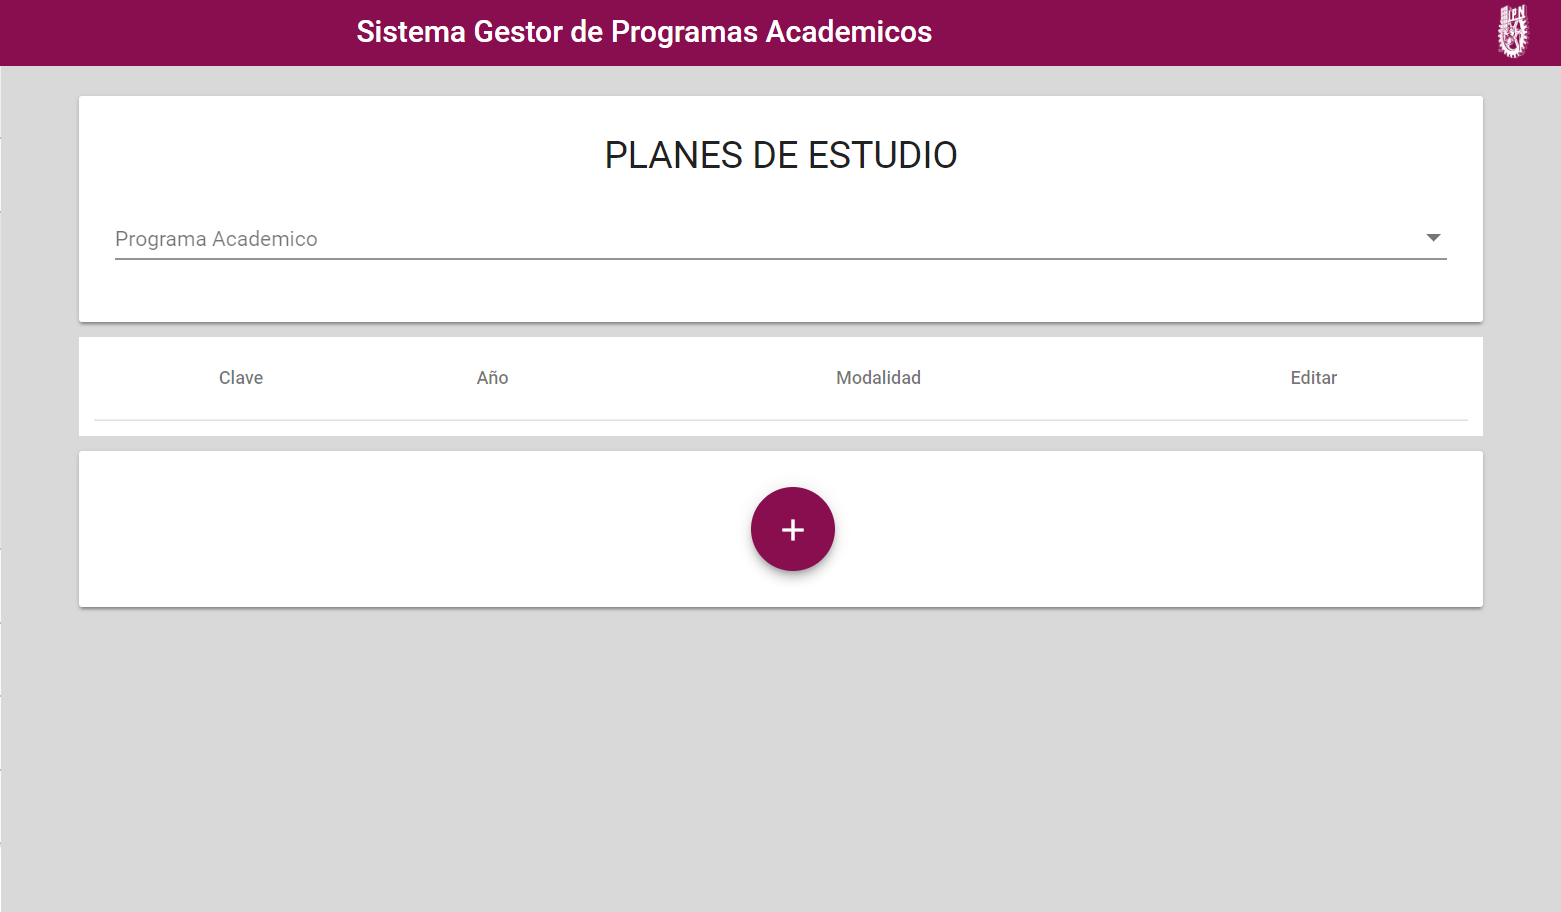
\includegraphics[width=0.7\linewidth]{images/SP4-GPE/consultar}}
	\caption{Pantalla para Planes de Estudio}
	\label{consultarPE}
\end{figure}

En donde aparecerá, de forma predeterminada, todos los Planes de Estudios a su cargo registrados en el sistema al momento. Tendrá a su disposición tres funciones:

\subsection{Buscar Planes de Estudio según su cargo}

Para ello, el Docente tendrá que seleccionar el Programa Académico que desea consultar en el siguiente componente:

\begin{figure}[!hbtp]
	\centering
	\hypertarget{academico}{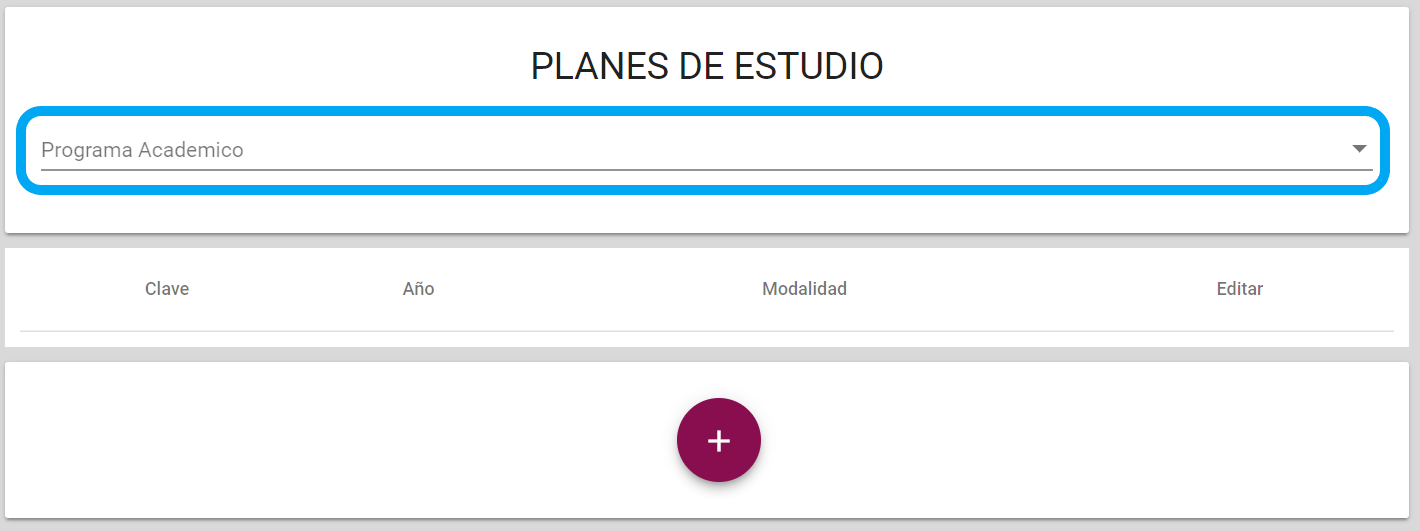
\includegraphics[width=0.7\linewidth]{images/SP4-GPE/programa}}
	\caption{Selección de Programa Académico}
	\label{academico}
\end{figure}

\begin{figure}[!hbtp]
	\centering
	\hypertarget{academico2}{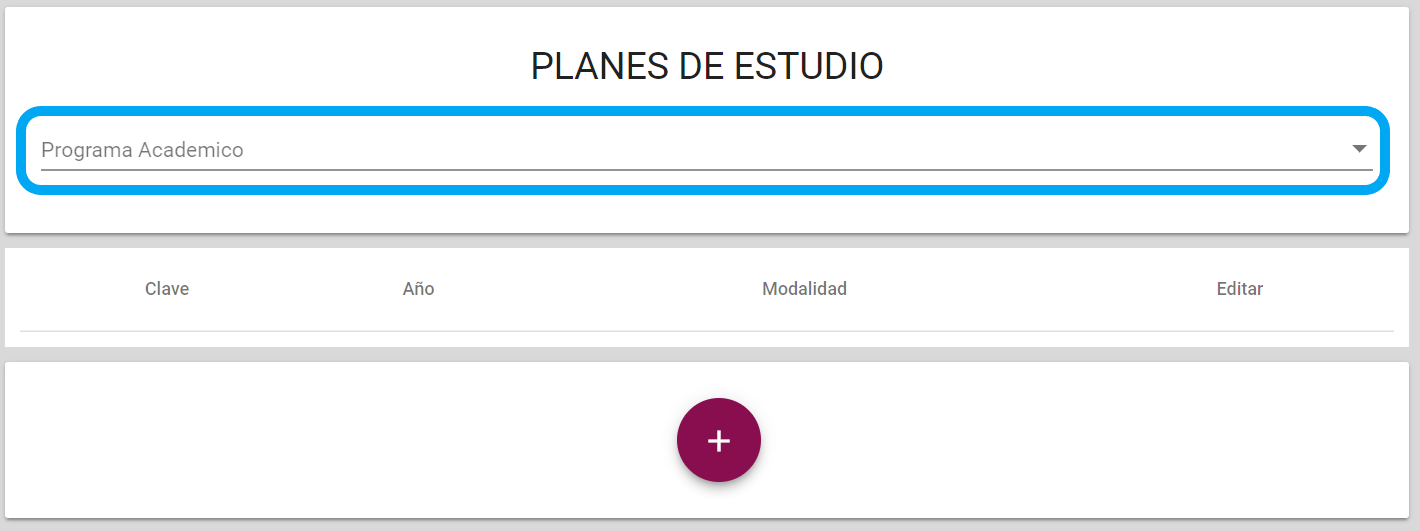
\includegraphics[width=0.7\linewidth]{images/SP4-GPE/programa}}
	\caption{Despliegue de Programas Académicos}
	\label{academico2}
\end{figure}

A continuación el sistema mostrará todos los Planes de Estudios que tengan el Programa Acádemico seleccionado.
\begin{figure}[!hbtp]
	\centering
	\hypertarget{planes}{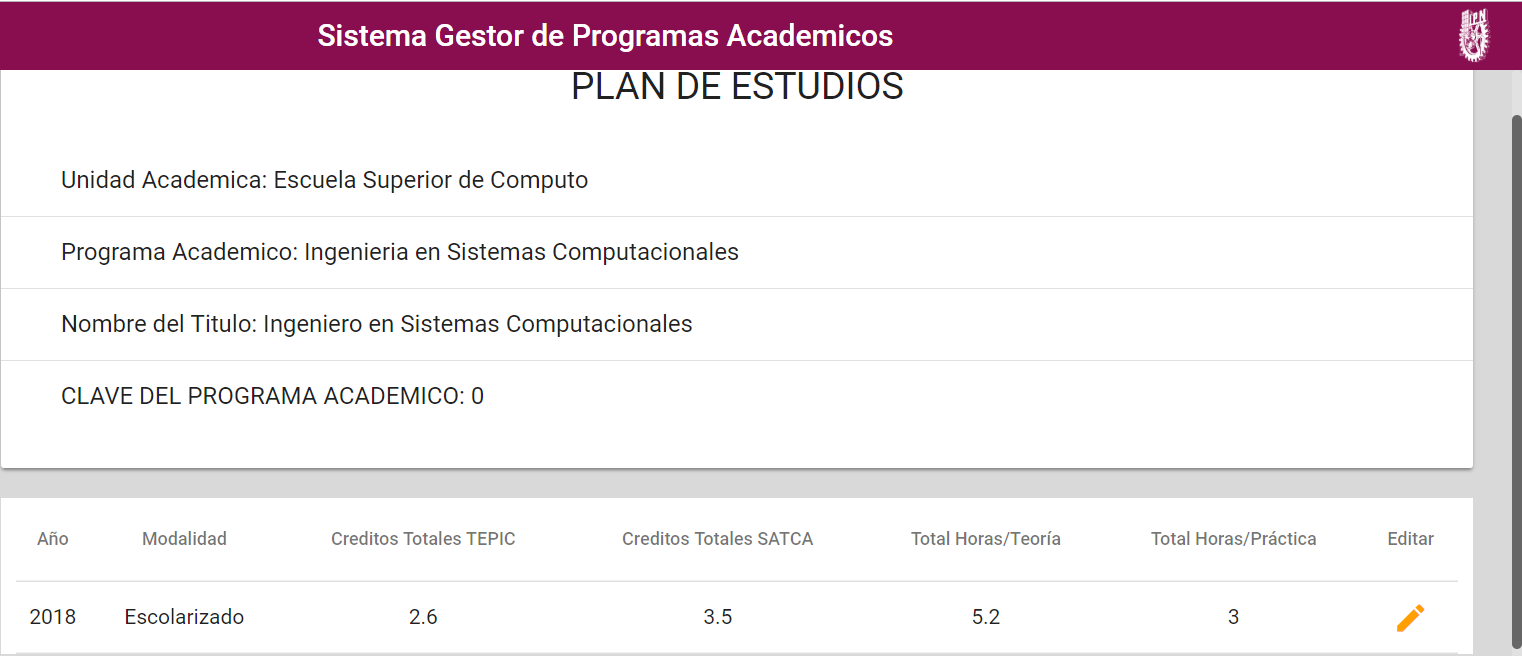
\includegraphics[width=0.7\linewidth]{images/SP4-GPE/planes}}
	\caption{Planes de Estudios Encontrados}
	\label{planes}
\end{figure}
\newpage
\subsection{Editar Planes de Estudios}

Para ello, el Docente tendrá que dar clic en el boton \IUbutton{icono de lapiz amarillo} que esta al lado del Plan de Estudio que desea modificar. Al hacer esto, el sistema redireccionará al usuario a la pantalla de \hyperlink{editarPE}{\textit{Editar Plan de Estudio}}.

\begin{figure}[!hbtp]
	\centering
	\hypertarget{editar}{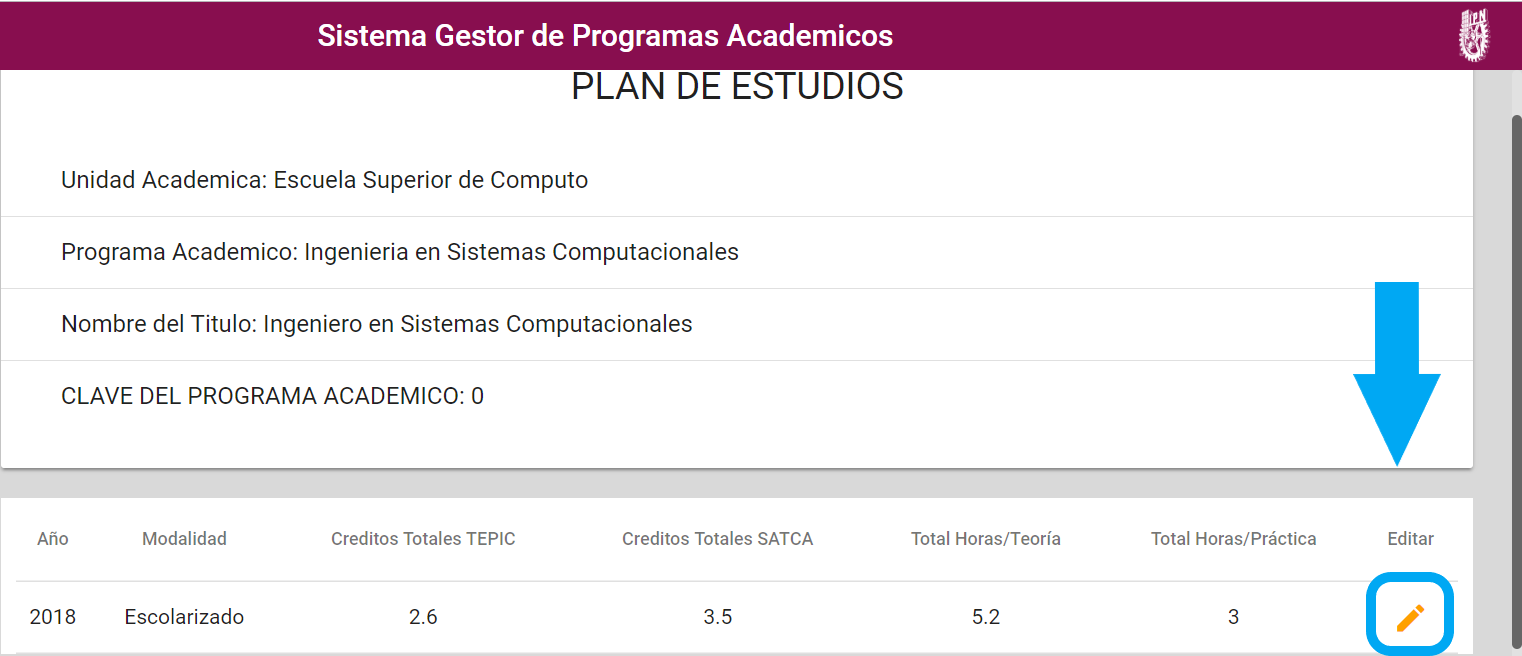
\includegraphics[width=0.7\linewidth]{images/SP4-GPE/editarC}}
	\caption{Botón Editar Plan de Estudio}
	\label{editar}
\end{figure}

\subsection{Registrar Planes de Estudios}

Para ello, el Docente tendrá que dar clic en el botón \IUbutton{+} en la parte inferior de la pantalla.

\begin{figure}[!hbtp]
	\centering
	\hypertarget{add}{
\includegraphics[width=0.7\linewidth]{images/SP4-GPE/mas}}
	\caption{Botón Agregar Plan de Estudio}
	\label{add}
\end{figure}

Al hacerlo, el sistema redireccionará al usuario a la pantalla de \hyperlink{registrarPE}{\textit{Registrar Plan de Estudio}}.


\textbf{NOTA:} En caso de que exista un error de conexión, aparecerá el siguiente mensaje:
%Imagen del MSG7

Al dar clic en en botón \IUbutton{Aceptar}, el sistema redireccionará al usuario a la pantalla de inicio. Debe esperar a que la página este disponible o intentar acceder nuevamente.


%-------------------------------------------------------------------------------------------------------
%-----------------------------REGISTRO DE PLANES DE ESTUDIO---------------------------------
%-------------------------------------------------------------------------------------------------------
\newpage

\section{Registro de Plan de Estudio}
Si el Docente en la pantalla de \hyperlink{consultarPE}{\textit{Consultar Planes de Estudios}} dio clic en el botón \IUbutton{+}, aparece la siguiente pantalla:

\begin{figure}[!hbtp]
	\centering
	\hypertarget{registrarPE}{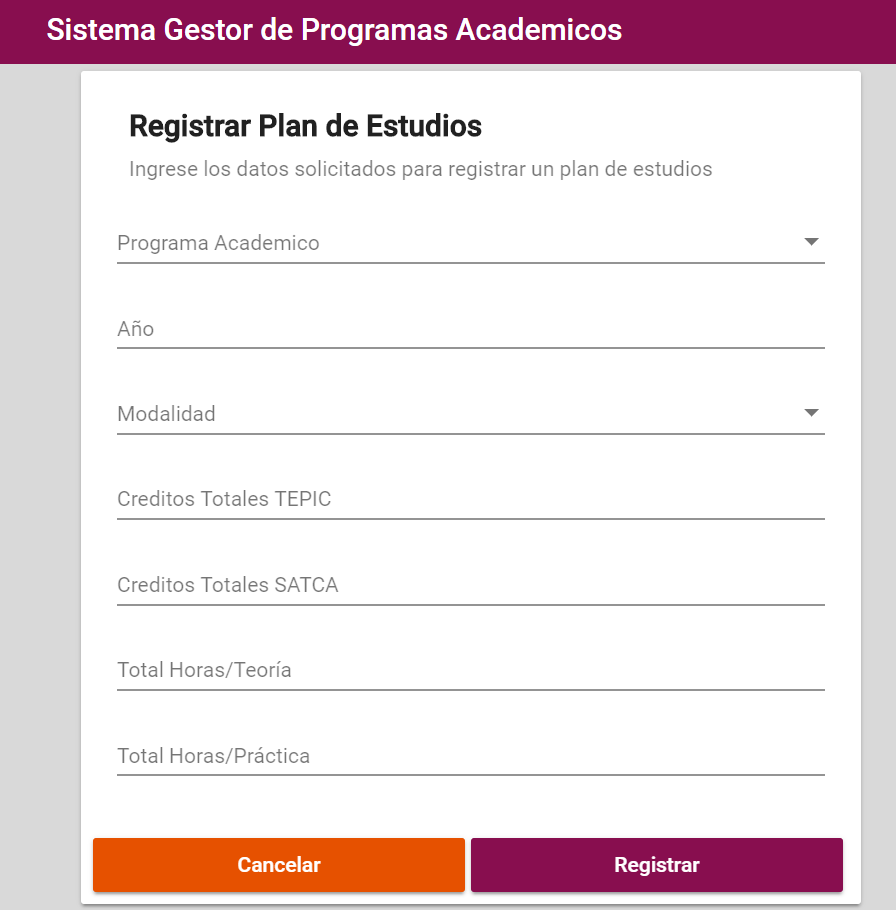
\includegraphics[width=0.7\linewidth]{images/SP4-GPE/registrarPE}}
	\caption{Pantalla para registrar Planes de Estudio}
	\label{registrarPE}
\end{figure}
\newpage
En donde tendrá que ingresar los campos del nuevo Plan de Estudio o en el formulario. Un ejemplo del llenado sería el siguiente:

\begin{figure}[!hbtp]
	\centering
	\hypertarget{ejreg}{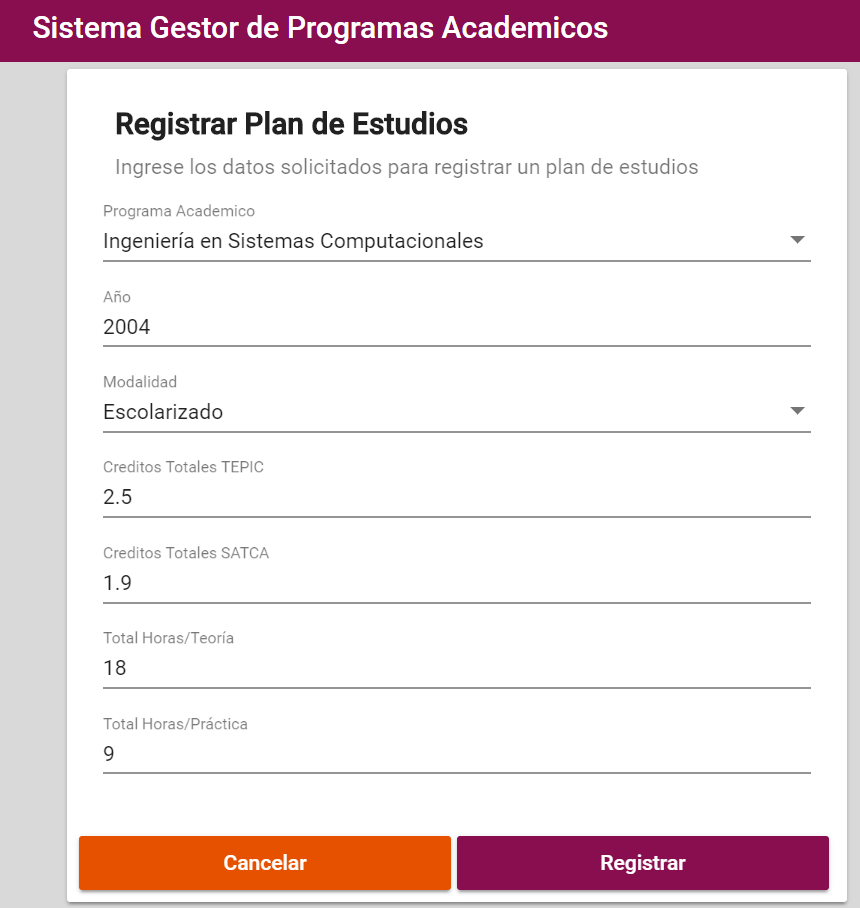
\includegraphics[width=0.7\linewidth]{images/SP4-GPE/registrarEjem}}
	\caption{Ejemplo de llenado para agregar un nuevo Plan de Estudios}
	\label{ejreg}
\end{figure}

\newpage
Si el Docente  da clic en el botón \IUbutton{Cancelar} sin haber concluido el registro del Plan de Estudio:

\begin{figure}[!hbtp]
	\centering
	\hypertarget{cancel2}{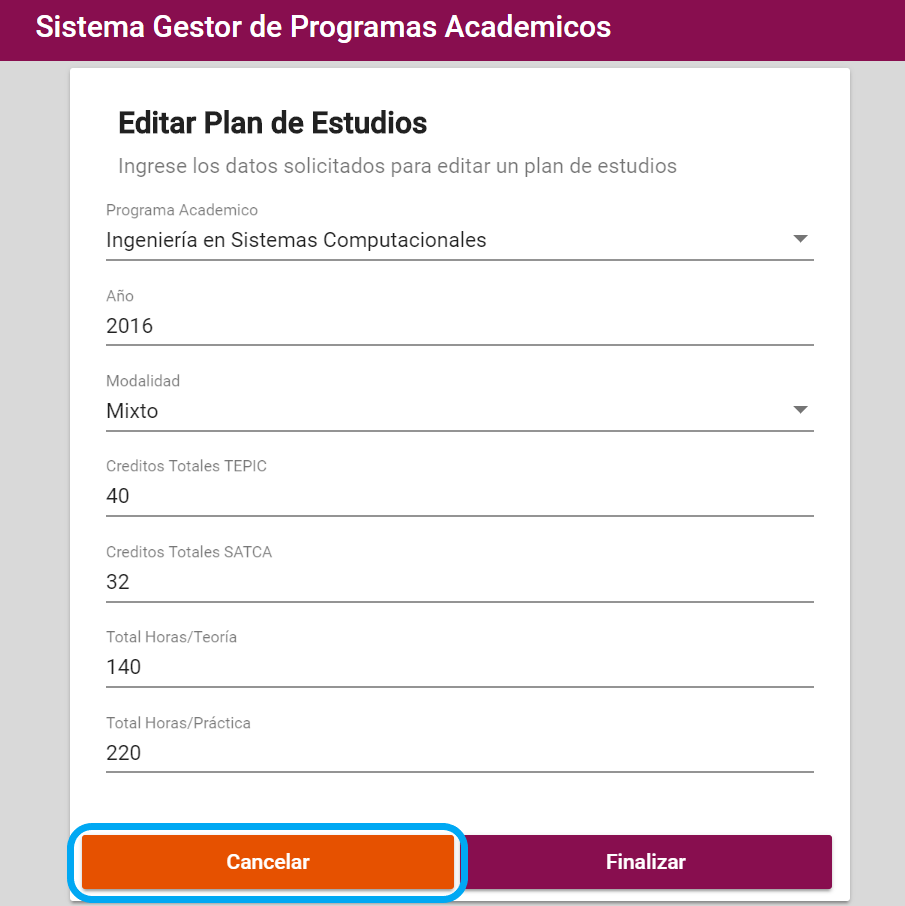
\includegraphics[width=0.7\linewidth]{images/SP4-GPE/cancelarPE}}
	\caption{Botón ''Cancelar''}
	\label{cancel2}
\end{figure}

El sistema mostrará el siguiente mensaje:
%Imagen MSG30

Para confirmar, el usuario debe dar clic en el botón  \IUbutton{Si}, y el Plan de Estudio no será registrado.\\

Para cancelar, el usuario debe dar clic en botón  \IUbutton{No}, el mensaje se cerrará y continuaremos en el formulario. Aqui el Docente puede terminar la edición del Plan de Estudio.\\
\newpage
A continuación, una vez verificados los datos, deberá de dar clic en el botón \IUbutton{Registrar}.
\begin{figure}[!hbtp]
	\centering
	\hypertarget{btnreg}{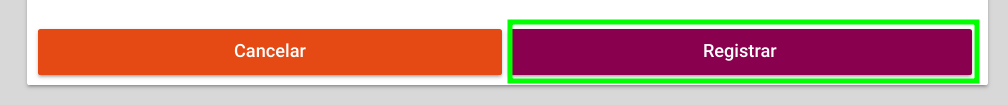
\includegraphics[width=0.7\linewidth]{images/SP4-GPE/registrarB}}
	\caption{Botón ''Registrar''}
	\label{btnreg}
\end{figure}

Si no hubieron errores, el sistema muestra el siguiente mensaje:
% Imagen MSG5

Al dar clic en en botón \IUbutton{Aceptar}, el sistema redireccionará al usuario a la pantalla de \hyperlink{consultarPE}{\textit{Consultar Planes de Estudios}}, en donde podrá ver el nuevo Plan de Estudios agregado.\\

\subsection{Posibles errores}
\begin{itemize}
	
	\item Problemas con la conexión o el sistema
	
	Si al momento de acceder a la pantalla de \hyperlink{registrarPE}{\textit{Registrar Plan de Estudios}} o al intentar registrar un Plan de Estuido, aparece alguno de los siguientes mensajes:
	%Imagen MSG7 Y MSG25
	
	Significa que existió un error de conexión o del sistema. Al dar clic en en botón \IUbutton{Aceptar}, el sistema redireccionará al usuario a la pantalla de \hyperlink{consultarPE}{\textit{Consultar Planes de Estudios}}. Debe esperar a que la página este disponible o intentar acceder nuevamente.
	
	\item Campos vacíos al momento de agregar un nuevo Plan de Estudio
	
	Si el Docente dejo en blanco algún campo del formulario, y posteriormente dio clic en el botón \IUbutton{Registrar}, el sistema mostrará el siguiente mensaje:
	%Imagen MSG32
	
	Al dar clic en botón \IUbutton{Aceptar}, el mensaje se cerrará y regresaremos al formulario, en donde el usuario deberá llenar el o los campos que dejo vacío. Si se continúan dejando campos en blanco y dando clic en el botón \IUbutton{Registrar}, aparecerá nuevamente el mensaje, hasta que todos los campos sean llenados.\\
	

	
	\item Los campos ingresados no son válidos
	
	Si al momento de dar clic en el botón \IUbutton{Registrar} aparece el siguiente mensaje:
	%Imagen MSG20

	
\end{itemize}
%-------------------------------------------------------------------------------------------------------
%-----------------------------EDICION DE PLANES DE ESTUDIOS--------------------------------
%-------------------------------------------------------------------------------------------------------

\newpage
\section{Edición de Planes de Estudios}
Si el  Docente en la pantalla de \hyperlink{consultarPE}{\textit{Consultar Planes de Estudios}} dio clicen el boton \IUbutton{icono de lapiz amarillo} de un Plan de Estudios, aparece la siguiente pantalla:

\begin{figure}[!hbtp]
	\centering
	\hypertarget{editarPE}{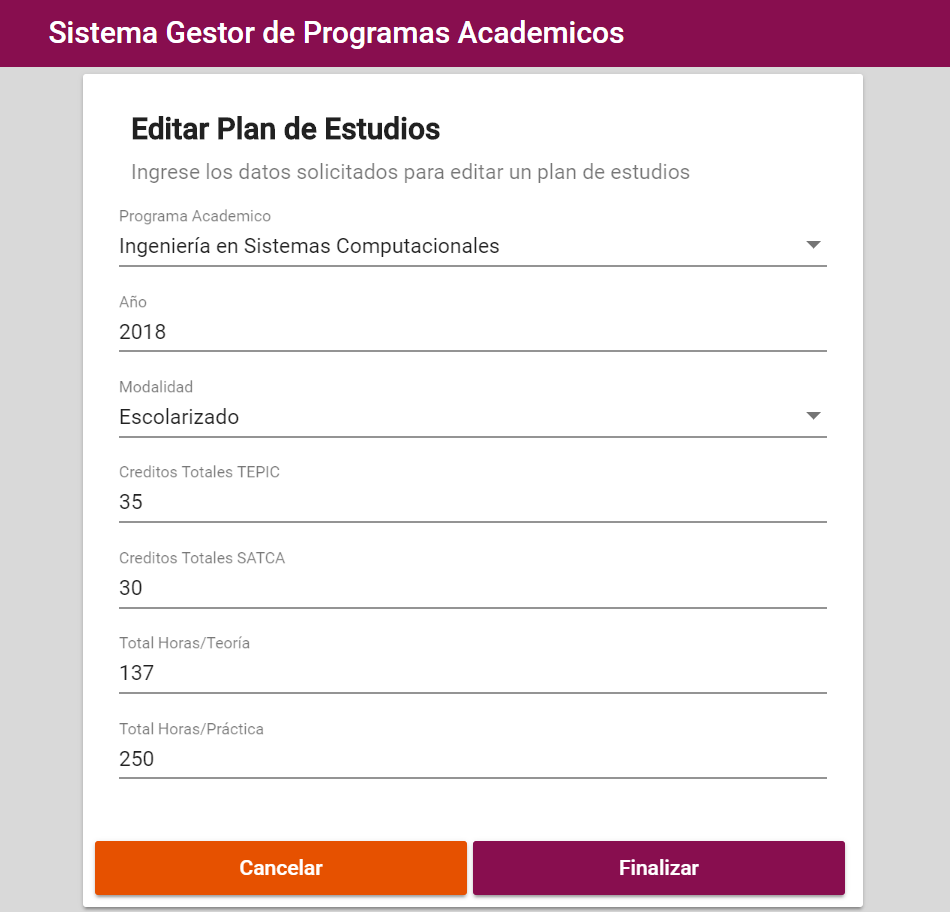
\includegraphics[width=0.7\linewidth]{images/SP4-GPE/editarPE}}
	\caption{Pantalla para la edición de Planes de Estudios}
	\label{editarPE}
\end{figure}

En donde se cargaran los datos del Plan de Estudio seleccionado en la pantalla de \hyperlink{consultarPE}{\textit{Consultar Planes de Estudios}} y llenará el formulario.\\
\newpage
Si el Docente  da clic en el botón \IUbutton{Cancelar} sin haber concluido el registro del Plan de Estudio:

\begin{figure}[!hbtp]
	\centering
	\hypertarget{cancel2}{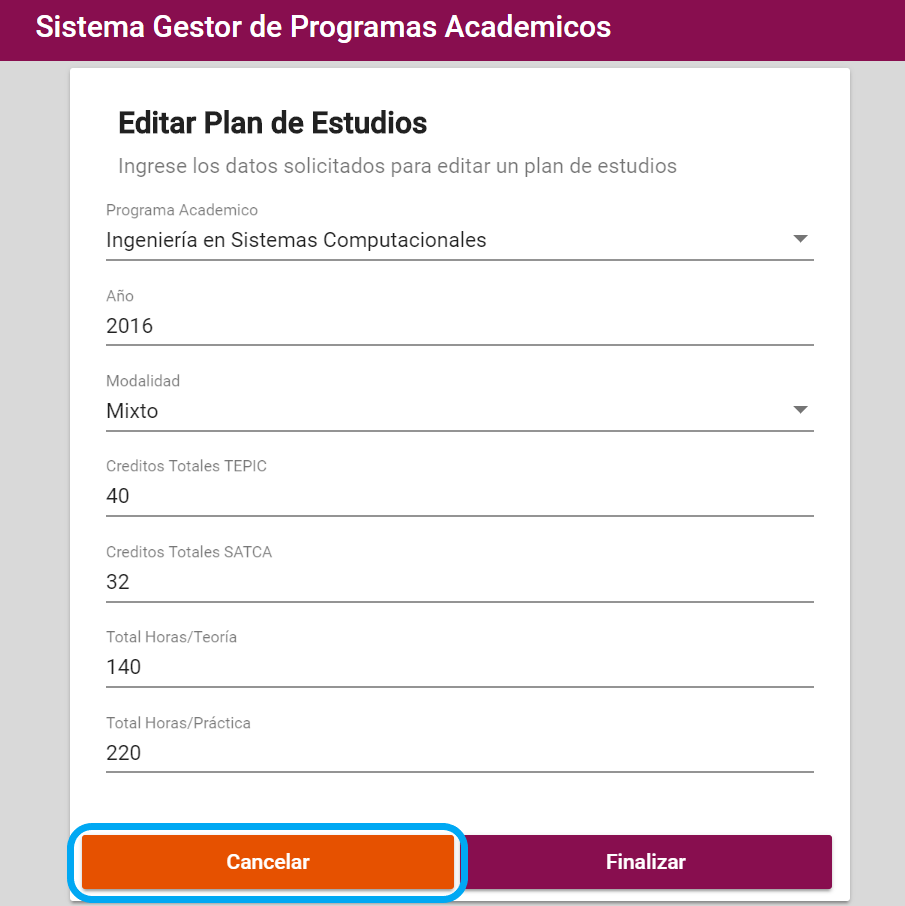
\includegraphics[width=0.7\linewidth]{images/SP4-GPE/cancelarPE}}
	\caption{Botón ''Cancelar''}
	\label{cancel2}
\end{figure}

El sistema mostrará el siguiente mensaje:
%Imagen MSG30

Para confirmar, el usuario debe dar clic en el botón  \IUbutton{Si}, y el Plan de Estudio no será registrado.\\

Para cancelar, el usuario debe dar clic en botón  \IUbutton{No}, el mensaje se cerrará y continuaremos en el formulario. Aqui el Docente puede terminar la edición del Plan de Estudio.\\
\newpage
A continuación, el usuario puede modificar todos los campos del Plan de Estudio:
\begin{figure}[!hbtp]
	\centering
	\hypertarget{modif}{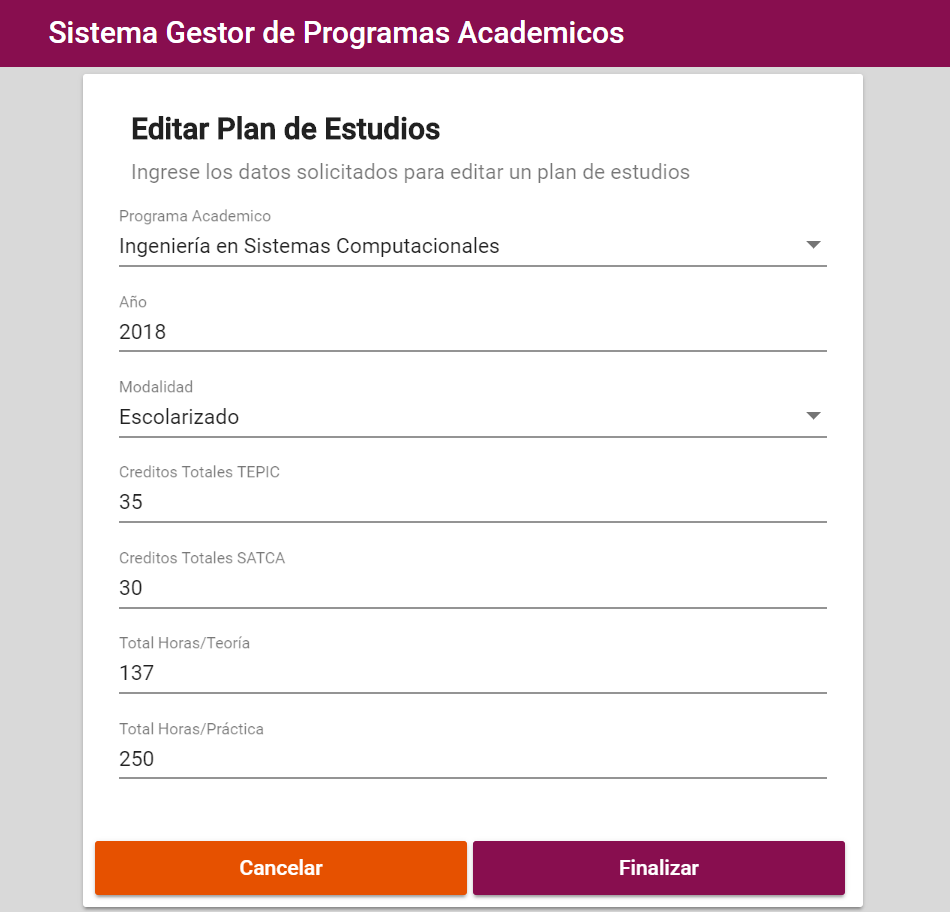
\includegraphics[width=0.7\linewidth]{images/SP4-GPE/editarPE}}
	\caption{Datos del Plan de Estudio modificados}
	\label{modif}
\end{figure}
\newpage

Una vez verificados los datos, deberá de dar clic en el botón  \IUbutton{Registrar}.
\begin{figure}[!hbtp]
	\centering
	\hypertarget{btnfin}{
\includegraphics[width=0.7\linewidth]{images/SP4-GPE/editarPER}}
	\caption{Botón ''Registrar''}
	\label{btnfin}
\end{figure}

Si no hubieron errores, el sistema muestra el siguiente mensaje:
%Imagen MSG27

Al dar clic en en botón  \IUbutton{Aceptar}, el sistema redireccionará al usuario a la pantalla de \hyperlink{consultarPE}{\textit{Consultar Planes de Estudis}}, en donde podrá ver las modificaciones del Plan de Estudios.\\

\subsection{Posibles errores}

\begin{itemize}
	\item Problemas con la conexión o el sistema
	
	Si al momento de acceder a la pantalla de \hyperlink{editarPE}{\textit{Editar Plan de Estudio}} o al intentar modificar un Plan de Estudio, aparece alguno de los siguientes mensajes:
	
	% Imagen MSG7 Y MSG25
	
	Significa que existió un error de conexión o del sistema. Al dar clic en en botón  \IUbutton{Aeptar}, el sistema redireccionará al usuario a la pantalla de \hyperlink{consultarPE}{\textit{Consultar Planes de Estudios}}. Debe esperar a que la página este disponible o intentar acceder nuevamente.
	
	\item Campos vacíos al momento de modificar el Plan de Estudio
	
	Si el Docente dejo en blanco algún campo del formulario, y posteriormente dio clic en el botón  \IUbutton{Registrar}, el sistema mostrará el siguiente mensaje:
	
	% Imagen MSG32
	
	Al dar clic en botón  \IUbutton{Aceptar}, el mensaje se cerrará y regresaremos al formulario, en donde el usuario deberá llenar el o los campos que dejo vacío. Si se continúan dejando campos en blanco y dando clic en el botón  \IUbutton{Registrar}, aparecerá nuevamente el mensaje, hasta que todos los campos sean llenados.
	
	\item Los campos ingresados no son válidos
	
	Si al momento de dar clic en el \IUbutton{Registrar} aparece el siguiente mensaje:
	% Imagen MSG20
	
	Significa que la composición de los datos ingresados en el formulario no es la correcta, verifíquelos e intente de nuevo.
	
\end{itemize}
